\documentclass{beamer}
\usepackage{ucltemplate}

%% Choose the color you like
\usecolortheme{blue}
\setbeamertemplate{navigation symbols}{}

%\AtBeginSection[] {
%  \begin{frame}
%    \frametitle{Outline}
%    \tableofcontents[currentsection]
%  \end{frame}
%}

%\usepackage[colorlinks=true]{hyperref}

\title{CNV calling, and a set of other useful notes}
\author[]{Vincent Plagnol}
\institute{
Inivata- Head of Computational Biology\\
UCL- Reader in Statistical Genetics\\
}
\date{}


\begin{document}

\maketitle





%%%%%%%%%%%%%%%%%%%%%%%

\begin{frame}
  \frametitle{Longer reads exist if you need them}
  \begin{center}
    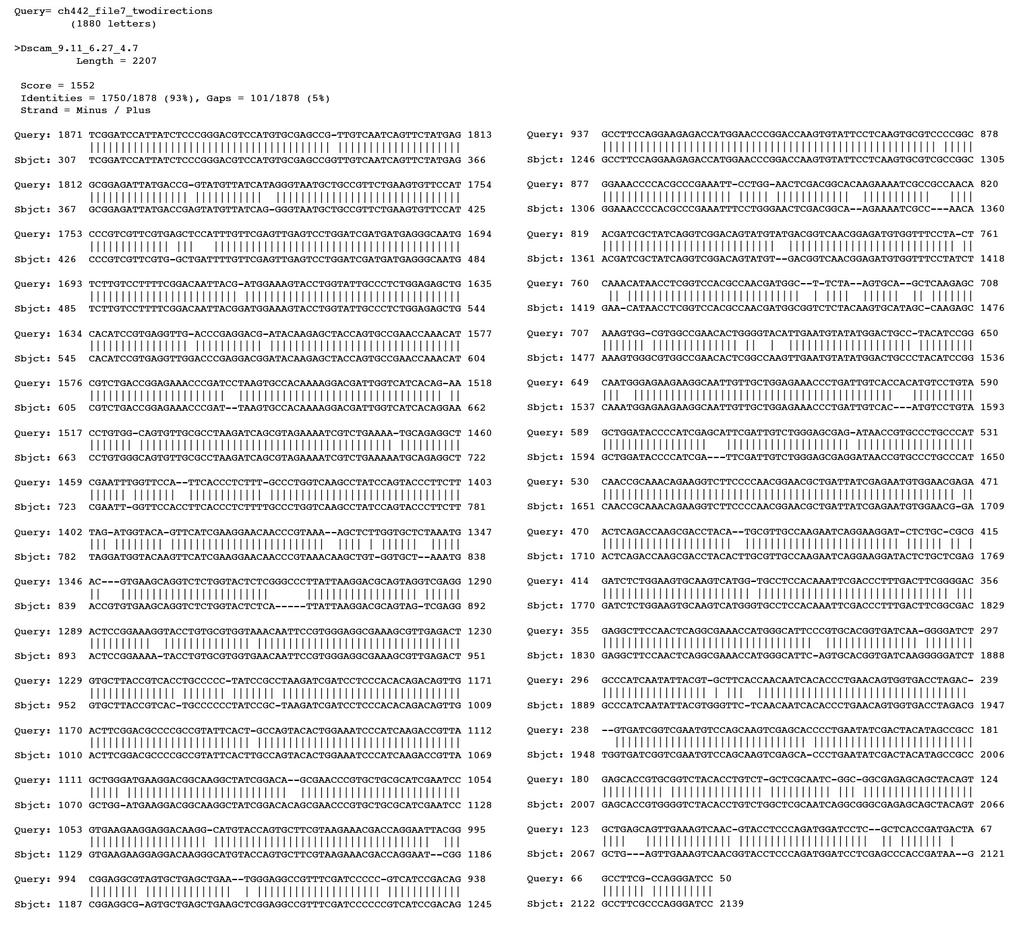
\includegraphics[width=10cm]{fig/nanopore.jpg}
  \end{center}
\end{frame}

\begin{frame}
  \frametitle{BEDtools: your swiss army knife for all issues}
  \begin{itemize}
  \item \href{http://bedtools.readthedocs.org/en/latest/}{BEDtools} is one of the most widely used tools in bioinformatics.
  \item It does tons of things, and while many look trivial, together they are very impressive.
  \item Well worth looking at what it can do, because it may solve many practical questions.
    \begin{itemize}
    \item In R, most routines are implemented within \texttt{GenomicRanges}, a bioconductor package.
    \end{itemize}
  \end{itemize}
\end{frame}


\begin{frame}
  \frametitle{Calling CNVs}
  \begin{itemize}
  \item There are many tools to call CNVs from sequence data, and I think you have already covered some of them.
  \item One option is read depth: excess of reads mark a duplication, too few reads mark deletions.
  \item But there are also specific read patterns, like reads mapping further apart than they should, that can mark a deletion.
  \item Split read is another way to go about it.
  \end{itemize}
\end{frame}


\begin{frame}
  \frametitle{An example of read depth based call in GATA2}
  \begin{center}
    \includegraphics[width=11cm]{fig/GATA2.pdf}
  \end{center}
\end{frame}


\begin{frame}
  \frametitle{Copy number variant analysis}
  \includegraphics[width=10cm]{fig/Lude.pdf}
\end{frame}



\end{document}
